\section{The White-Box Model}\label{sec:whiteBoxModel2}

We can imagine the components of the mind as white boxes which inform other components by their very functioning --- however, this does not lend itself to easy implementation. Instead, we can emulate this behaviour via a \caps{message space}, from which individual components take their input and into which they put their output. A \caps{component} is then a local processing unit which continuously scans the message space, running messages through its \caps{filter}. If the filter detects a relevant message, it is then passed to the \caps{interpreter}, which parses the message into the needed format and hands it over to the \caps{processor}. The processor, after having finished, puts its output back into the message space for other components to read. Figure~\ref{fig:global} illustrates this scheme. Note the lack of explicit hierarchical structure and central organising units.

\begin{figure}
	\begin{center}
		\begin{tabular}{l l}
			\toprule
			Symbol & Description\\
			\midrule
			
			\begin{minipage}[t]{0.2\textwidth}
				
\includegraphics[width=80pt]{Figs/legend_proc.png}
			\end{minipage}
			& Processing component\\
			
\includegraphics[width=80pt]{Figs/legend_choice.png} & Choice\\
			
\includegraphics[width=50pt]{Figs/legend_container.png} & Data container (Queue, List, etc.)\\
			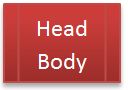
\includegraphics[width=50pt]{Figs/legend_data.png} & Data\\
			
\includegraphics[width=30pt]{Figs/legend_generator.png} & Stream generator\\
			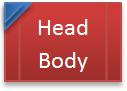
\includegraphics[width=50pt]{Figs/legend_imaginary.png} & Counterfactual (imaginary) data\\
			\bottomrule
		\end{tabular}
	\end{center}
	\caption{Notation for the diagrams in this and the following sections.}
	\label{fig:diagramNotation}
\end{figure}
%
\begin{figure}[!h]
	\centering
	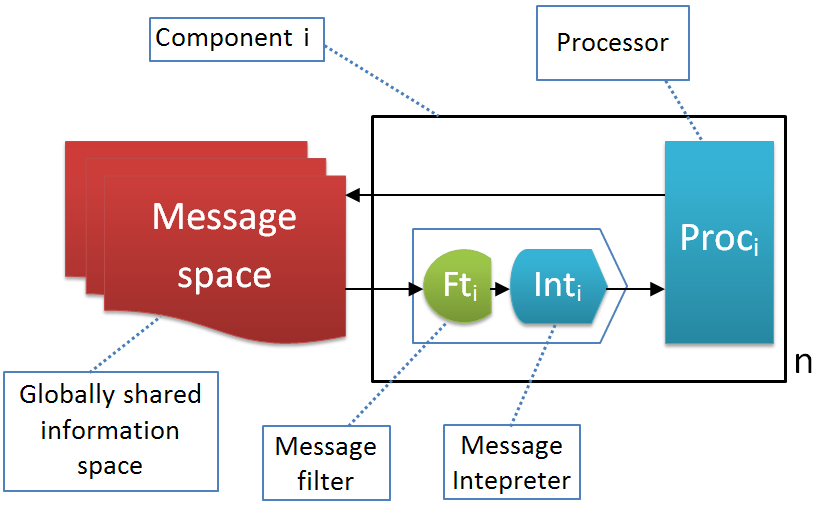
\includegraphics[width=400pt]{Figs/global.png}
	\caption{Global neural architecture.}
	\label{fig:global}
\end{figure}

However, as I'll show in the next section, this model is generic enough to accommodate such special-purpose structures. Figure~\ref{fig:global} shows the message-passing scheme, but it also specifies a graph in which the nodes are the components and fixed, while the edges are the accepted messages and are determined by the nodes; through their filters, components control the shape of the graph. By imposing invariants on these filters, we can have the graph take any shape we desire. In particular, we can model the kinds of structures that occur in many other cognitive models and in empirical research: central organisers, sequences of components (``pipelines''), localized messages affecting only a small part of the mind, a component reading its own messages, loops and iterative messages between two or more components et cetera.

\pagebreak

\paragraph{Messages.}

We may now ask how such messages between components are structured. Here, I make two empirical claims:
\begin{enumerate}
	\item messages have a priority and
	\item they are effectively unstructured.
\end{enumerate}

\begin{figure}[!h]
	\centering
	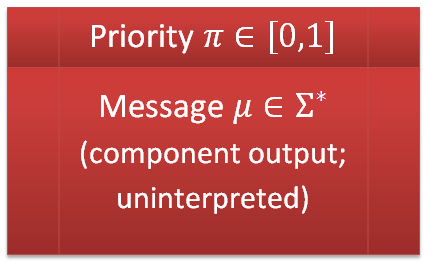
\includegraphics[width=150pt]{Figs/message.png}
	\caption{Structure of a neural message.}
	\label{fig:message}
\end{figure}

To the best of my knowledge, the veracity of either has thus far not been determined by neuroscience. For the first, Marvin Minsky's ``The Emotion Machine'' provides some circumstantial evidence \cite[p. 222]{emotionMachine}:

\begin{quote}
	Of course, when one activates two or more Critics or Selectors, this is likely to cause some conflicts, because two different resources might try to turn on a third resource both {\em on} and {\em off}. To deal with this, we could design the system to use various policies like these:
	
	\begin{enumerate}
		\item Choose the resource with the highest priority.
		\item Choose the one that is most strongly aroused.
		\item Choose the one that gives the most specific advice.
		\item Have them all compete in some ``marketplace''.
	\end{enumerate}
\end{quote}

The selection strategies Minsky lists imply that there is some mechanism in the brain to determine the urgency of a signal. While it is possible that higher brain functions like reasoning or affect make an additional, rational evaluation, sensations like intense pain, bright lights, or great sadness can likely be communicated most easily by the appropriate components causing a flood of activity which, by its very intensity, informs other components of the urgency of their messages.

The second claim --- that messages are essentially unstructured --- means that there is no common, agreed-upon format in which they are stored. In addition to the evolutionary implausibility of such a format being created, an unstructured message format is in line with the white-box nature of components: since components merely ``listen in'' on others, and since each components will have its own pattern of activity, a listener would simply have to try and make sense of this activity as best it could. The proposed structure of messages is thus shown in Figure~\ref{fig:message}: every message comprises a priority header, together with an unstructured body which, for our purposes, is simply a string of bits.

\paragraph{Filters.} Before a component can respond to a message by another, such a message must be assessed for the presence of relevant information. Conceptually, this happens via a \caps{filter} in each component, which pattern-matches incoming messages and, if a certain threshold is reached, signals relevance and hands the message over the \caps{interpreter} for parsing. Figure~\ref{fig:filter} shows such a filter: it is composed of a directed graph of nodes, and a node is activated if it detects some specific content in the message. Nodes, in turn, are connected via edges of strength $\in [0,1]$. When a node is activated, it sends a charge proportional to the strength of its link to its neighbours, contributing to their activation as well. Some nodes are marked as {\em output nodes}; if enough such output nodes become activated, the message is deemed to be sufficiently relevant. This model of filters is inspired by the {\em spiking neural P Systems} of Georghe Pa\u{u}n et al. (\cite[p. 337]{membraneComputing} and \cite{spikingNeural}), in which charges sent along directed graphs of neurons are used to compute functions.

\begin{figure}[!h]
	\centering
	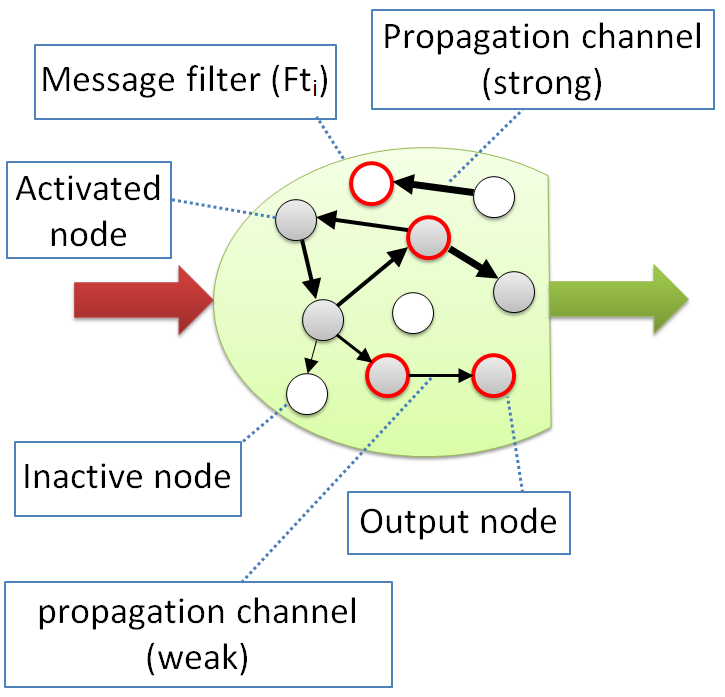
\includegraphics[width=168pt]{Figs/filter.png}
	\caption{A pattern-matching filter for a component $C_i$.}
	\label{fig:filter}
\end{figure}

\section{Mathematical Model}\label{sec:mathematicalModel}

We now create a mathematical model for the description of the architecture. This model will be split into two parts: the structural and the operational semantics. The structural semantics encode the static properties of neural systems, whereas the operational semantics describe the behaviour of such a system at runtime.

\subsection{Preliminaries}\label{sec:mathematicalPreliminaries}

Since the mathematical model is built with implementation in mind, I will use some basic type theory in the coming sections. The following notions are from the $\lambda$-calculus and its attendant type systems; anyone familiar with such can therefore freely skip this section. We will introduce types, type constructors, and their relation to functions, together with a few example types which will come in handy later on. The following can be found in any introduction to type theory and was taken (with simplification) from \cite{Mendler:1988:IDT:913822}, \cite{typeIntroduction2}, and \cite{Jacobs97atutorial}.

\begin{definition}[Syntax: Type]\label{def:type}
	For our purposes, types are defined inductively thus:
	\begin{description}
		\item[Basic type.] $\R$ and $\emptyset$ are types.
		\item[Sum type.] If $\type{T_1},\type{T_2}$ are types, the {\em sum type} $\type{T_1 + T_2}$, is a type. 
		\item[Product type.] If $\type{s}$ is a string and $\type{T_1},\dots,\type{T_n}$ are types, the {\em product type} $\type{s}\ \type{T_1} \dots \type{T_n}$, is a type. A special case is the {\em anonymous product type} \paren{tuple}, where $s=``\langle\rangle"$. There, we just write $\langle\type{T_1},\dots,T_n \rangle$.
		\item[Full application.] If $\type{T_1},\dots,\type{T_n}$ are types and $\allQ{x_1,\dots,x_n} \type{C}$ is a type constructor \paren{see next definition}, then $\type{C\ T_1} \dots \type{T_n}$, is a type.
		\item[$\mu$-abstraction.] If $\type{T}, \type{S}$ are types and $\type{S}$ occurs in $\type{T}$, then $\muQ{\alpha}\type{T}[\type{S}\backslash\alpha]$ \paren{for a fresh variable name $\alpha$} is a type.
	\end{description}
\end{definition}

\begin{definition}[Syntax: Type constructor]\label{def:typeCon}\
	Type constructors are the defined thus:
	\begin{description}
		\item[Base case.] Every type $\type{T}$ is a type constructor.
		\item[Abstraction.] If $\type{C}$ is a type constructor and $\type{T}$ is a type, $\allQ{x} \type{C}[\type{T}\backslash x]$ is a type constructor.
		\item[Sum types.] If $\type{C_1}\dots,\type{C_n}$ are type constructors with $\type{C_i} = \allQ{x^i_1\dots,x^i_n} \type{T_i}$ \paren{$1 \leq i \leq n$}, then\\ $\allQ{x_1,\dots,x_n} (\type{C_1} + \dots + \type{C_n})$ is a type constructor.
		\item[Partial application.] If $\type{T_1},\dots,\type{T_i}$ \paren{$i < n$} are types and $\allQ{x_1,\dots,x_n} \type{T}$ is a type constructor,\\ then $\allQ{x_{i+1},\dots,x_n} \type{T}[x_1\backslash \type{T_1},\dots,x_i\backslash \type{T_i}]$ is a type constructor.
	\end{description}
\end{definition}

Every type is interpreted as a set of values which are of that type; type constructors are interpreted as universally quantified templates for actual types. Their formal semantics are as follows:

\begin{definition}[Semantics: Type]\label{def:typeSem}
	Let $\type{T}$ be a type. Its interpretation function $\tint(\type{T})$ is defined thus:.
	\begin{description}
		\item[Basic type.] $\R$ is interpreted as the set of real numbers. $\tint(\emptyset) = \{\}$.
		\item[Sum type.] If $\type{T_1}, \type{T_2}$ are types, then $\tint(\type{T_1 + T_2}) = \tint(\type{T_1}) \cup \tint(\type{T_2})$.
		\item[Product type.] If $\type{T_1},\dots,\type{T_n}$ are types and $\type{s}$ is a string, then
		$$
		\tint(\type{s}\ \type{T_1} \dots \type{T_n}) = \left\{
		\begin{array}{l l}
		\{\type{s}\} & \mt{if } n = 0\\
		\{\type{s}\} \times \tint(\type{T_1}) \times \dots \times \tint(\type{T_n}) & \mt{if } n \geq 1.
		\end{array}
		\right.
		$$
		
		\item[Full application.] If $\type{T_1},\dots,\type{T_n}$ are types and $\allQ{x_1,\dots,x_n} \type{C}$ is a type constructor, then
		$$
		\tint(\type{C}\ \type{T_1} \dots \type{T_n}) = \bigcup\limits_{v_1 \in\ \tint(\type{T_1})} \cdots \bigcup\limits_{v_n \in\ \tint(\type{T_n})} \left( \bigcup\limits_{C' \in\ \cint(C)} C'[x_1\backslash v_1,\dots, x_n\backslash v_n] \right).
		$$
		
		\item[$\mu$-abstraction.] If $\muQ{\alpha}\type{T}$ is a type, then $$\tint(\muQ{\alpha}\type{T}) = \tint(\type{T}) \cup \tint(\type{T}[\alpha\backslash\type{T}]) \cup \tint(\type{T}[\alpha\backslash\type{T}][\alpha\backslash\type{T}]) \cup \dots$$
		
		with $\tint(\alpha) = \{\}$.
	\end{description}
\end{definition}

\begin{definition}[Semantics: Type constructor]\label{def:typeConSem}
	The partial interpretation function $\cint$ for type constructors is defined as follows: if $\type{C}$ is a type constructor containing exactly the types $\type{T_1},\dots,\type{T_n}$, then
	$$
	\cint(\type{C}) = \bigcup\limits_{v_1 \in\ \tint(\type{T_1})} \cdots \bigcup\limits_{v_n \in\ \tint(\type{T_n})} \type{C}[\type{T_1}\backslash v_1,\dots,\type{T_n}\backslash v_n].
	$$
\end{definition}

Intuitively, sum types are simply unions, product types are named cartesian products, and full applications are instantiations of type constructors with all possible values. $\mu$-abstraction represents recursive data types such as lists or trees. Type constructors themselves are just generic types.

Whenever we want to assert that an expression has a specific type, we write:

\begin{notation}[Typed expressions]
	Let $x$ be an expression and $\type{T}$ a type. $x :: \type{T}$ asserts that $x$ has type $\type{T}$.
\end{notation}

Henceforth, by convention, we will write type variables in lower-case and concrete types in upper-case, omitting the explicit $\forall$-blocks. That is, a type like $\allQ{x,y,z} \type{C\ x\ (\N + T_1)\ y\ z}$ will simply be written as $\type{C\ x\ (\N + T_1)\ y\ z}$ and it will be clear that $\type{x}, \type{y}, \type{z}$ are type variables, while $\N, \type{T_1}$ are concrete types. A special kind of type constructor is the function arrow ($\rightarrow$) which induces the function type:

\begin{example}[Function arrow]
	If we take, say, the type $\rightarrow \type{S1}\ \type{S2}$ (a product type with the product types $\type{S1}$ and $\type{S2}$ as arguments) and abstract twice, we get $\allQ{s,t} \rightarrow \type{s}\ \type{t}$. $\rightarrow \type{s}\ \type{t}$ is the type constructor for unary functions from $\type{s}$ to $\type{t}$, also written infix as $\type{s} \rightarrow \type{t}$. Functions with multiple arguments, mapping $\type{t_1},\dots,\type{t_{n-1}}$ to $\type{t_n}$, can be modelled in two ways: either through n-tuples, or through nested function arrows:
	
	$$
	\begin{array}{l}
	\tuple{\type{t_1}, \type{t_2}, \dots \type{t_{n-1}}} \rightarrow \type{t_n}\\
	\type{t_1} \rightarrow (\type{t_2} \rightarrow \dots \rightarrow (\type{t_{n-1}} \rightarrow \type{t_n})\cdots)
	\end{array}
	$$
	
	The first method necessitates that we supply all arguments at once, whereas the second allows them to be given one after another.
\end{example}

\noindent
Function arrows allow the execution of functions in the obvious way:

\begin{definition}[Function application]
	Let $f :: \type{S} \rightarrow \type{T}$ and $x$ be an expression of type $\type{S}$. Then $f\ x$ is an expression of type $\type{T}$. Function application associates to the left, that is: $f\ x_1 \dots x_n = (\cdots((f\ x_1)\ x_2) \dots x_n)$.
\end{definition}

\noindent
We can combine type constructors, sum types, and product types into {\em algebraic data types} (ADTs).

\begin{definition}[Algebraic data type (ADT)]\label{def:ADT}
	Let $\type{s}$ be a string and $\type{C_1},\dots,\type{C_n}$ be type constructors such that $\type{C_i} = \allQ{x_1,\dots,x_n} \type{T_i}$ and $\type{T_i}$ is a named product type with type variables \paren{$1 \leq i \leq n$}. Then $\allQ{x_1,\dots,x_n} (\type{T_i} + \dots + \type{T_n})$ is an ADT. If we want to give a name to an ADT, we write it as $\type{s\ x_1 \dots x_n = T_i + \dots + T_n}$.
\end{definition}

Since an ADT is merely the sum of product types, it is itself a type constructor. If it has no type variables, it is also a type. Next, we define a couple of example ADTs, some of which we will use in the next section.

\begin{example}[$\N$, $\B$, $\Q$, $\C$,  Maybe, Either, List]
	$$
	\begin{array}{l c l}
	\N & = & \muQ{\alpha}\type{Z + S\ \alpha}\\ 
	\B & = & \type{False + True}\\
	\Q & = & \type{Rat}\ \N\ \N\\
	\C & = & \type{Complex}\ \R\ \R\\
	\type{Maybe\ t} & = & \type{Nothing + Just\ t}\\
	\type{Either\ l\ r} & = & \type{Left\ l + Right\ r}\\
	\type{List\ a} & = & \muQ{\alpha}\ \type{Nil + (a : \alpha)}\\
	\end{array}
	$$
	
	$\N$ is the usual Peano definition of natural numbers, with a nullary product type $\type{Z}$ representing zero, and a unary product type $\type{S}$, which allows recursion. $\B$, $\Q$, $\C$ are the sets of Boolean number and rational/complex numbers, respectively, with $\type{False}$ and $\type{True}$ being nullary product types, and with $\type{Rat}\ \N\ \N$ and $\type{Complex}\ \R\ \R$ being binary ones. $\mathtt{Maybe}$ represents an optional value, which may or may not be present. $\mathtt{Either}$ represents a choice between two values, of which either the left or the right one is present, but not both. $\type{List\ a}$ \paren{or just $\type{[a]}$ as a shorthand} denotes a list of values of type $\type{a}$. There, $\type{Nil}$ is the nullary type constructor for an empty list and $\type{:}$ is an infix binary type constructor that stores the head and tail of a list.
\end{example}

\noindent
We also define the usual convenience functions for these types:
$$
\begin{array}{l l}
\begin{array}{r c l}
\field{isJust} & :: & \type{Maybe\ a \rightarrow Bool}\\
\field{isJust}\ m & = & \left\{
\begin{array}{l l}
\type{True} & \mt{if } m = \type{Just}\ x\\
\type{False} & \mt{otherwise}\\
\end{array}
\right.\\
\\
\field{fromJust} & :: & \type{Maybe\ a \rightarrow a}\\
\field{fromJust}\ m & = & \left\{
\begin{array}{l l}
x & \mt{if } m = \type{Just}\ x\\
\bot & \mt{otherwise}\\
\end{array}
\right.\\
\end{array}
&
\begin{array}{r c l}
\field{head} & :: & \type{[a] \rightarrow a}\\
\field{head}\ l & = & \left\{
\begin{array}{l l}
x & \mt{if } l = x:xs\\
\bot & \mt{otherwise}\\
\end{array}
\right.\\
\\
\field{tail} & :: & \type{[a] \rightarrow [a]}\\
\field{tail}\ l & = & \left\{
\begin{array}{l l}
xs & \mt{if } l = x:xs\\
\bot & \mt{otherwise}\\
\end{array}
\right.\\
\end{array}
\end{array}
$$

Definitions~\ref{def:type}--\ref{def:ADT} specify a fragment of System F$_\omega$,\footnote{Specifically, the decidable fragment of System F$_\omega$ without higher kinds and only prenex-polymorphism. That is, type constructors can only take types as arguments and are of the form $\allQ{x_1,\dots,x_n} \type{C}$ for quantifier-free $\type{C}$. This is also called the Hindley-Milner type system. For details, see \cite{barendregt91}.} which is used to type expressions in the lambda calculus. Although System F$_\omega$ is strictly more powerful, our definitions are enough to provide a description language for the data types and functions in the rest of this work.


\subsection{Neural Systems}\label{sec:mathematicalNeuralSystem}

\begin{definition}[Neural component]
	Let $I$ be an index set and let $\type{T}$ be any type. Then, a neural component $C$ with a name from $I$ and message type $\type{T}$ is a four-tuple
	$$
	\tuple{\field{name}, \field{ft}, \field{int}, \field{proc}}
	$$
	where
	\begin{enumerate}
		\item $\field{name} :: I$ is the {\em name} of $C$,
		\item $\field{ft} :: \type{T \rightarrow \B}$ is  called the {\em filter} of $C$,
		\item $\field{int} :: \type{T} \rightarrow \type{Maybe\ T}$ is called the {\em interpreter} of $C$, and
		\item $\field{proc} :: \type{T} \rightarrow \type{T}$ is called the {\em processor} of $C$.
	\end{enumerate}
	
	Formally, the type of $C$ is $\field{Comp}_{\type{T},I}$. As a shorthand, we denote the name, filter, interpreter and processor of a given component $C$ as $\field{name}_C$, $\field{ft}_C$, $\field{int}_C$, $\field{proc}_C$, respectively.
\end{definition}

\noindent
A set of neural components, together with a set of messages, induces a {\em neural system}:

\begin{definition}[Neural system]
	Let $T$ be any type and let $I$ be an index set. Then, a neural system with message type $T$ and component names from $I$ is a tuple
	$$
	\langle \textbf{Co}, \textbf{Me} \rangle
	$$
	where
	\begin{itemize}
		\item $\textbf{Co}$ is a set of neural components (with message type $T$ and names from $I$) and
		\item $\textbf{Me}$ is a set of elements of type $T$, called the {\em set of messages}.
	\end{itemize}
\end{definition}

\subsection{Sending and Receiving Messages}\label{sec:notation}

We now give a notation for the sending and receiving of messages in a system. Here, we distinguish two aspects: first, the structural, which describes how messages {\em can} travel in a system and the operational, which describes how they {\em do} travel in some given scenario.

\subsubsection{Structural Notation}

The elements of a component statically determine which messages it can receive and send. Based on the behaviour of the filter, interpreter and processor of a component, we can express a number of properties.

\begin{definition}[Message reception]
	Let $C$ be a component and $m$ a message. $C$ can receive $m$ if and only if $\ft{C}\ m = \field{True}$ and $\int{C}\ m = \field{Just}\ m'$ for some $m'$.
	When $C$ can receive all messages in $\{m_1,\dots,m_n\}$, we write:
	$$
	\canrec{m_1,\dots,m_n}{C}.
	$$
	
	We denote the opposite statement --- that $C$ cannot receive any message in $\{m_1,\dots,m_n\}$ --- by:
	
	$$
	\cantrec{m_1,\dots,m_n}{C}.
	$$
\end{definition}

\begin{definition}[Message sending]
	Let $C$ be a component and $m, m_1,\dots,m_n$ messages. $C$ can send out a message $m$ if and only if there exists a message $m_{\mt{in}}$ s.t. $\proc{C}\ m_{\mt{in}} = m$.
	When $C$ can send all messages in $\{m_1,\dots,m_n\}$, we write:
	
	$$
	\cansend{C}{m_1,\dots,m_n}.
	$$
	
	The opposite statement --- that $C$ cannot send any message in $\{m_1,\dots,m_n\}$ --- is denoted by:
	$$
	\cantsend{m_1,\dots,m_n}{C}.
	$$
\end{definition}

\begin{definition}[Receiving set]
	The set of components which can receive a message $m$ is denoted by
	
	$$
	\rec{m} \equiv \{C \in \co\ |\ \canrec{m}{C} \}.
	$$
	
	$\field{rec}$ can also be overloaded to refer to the set of components which can receive and interpret at least some message of a component $C$:
	
	$$
	\rec{C} \equiv \{C_i \in \co\ |\ \exists m:\ \cansend{C}{m} \wedge \canrec{m}{C_i} \}.
	$$
\end{definition}


\subsubsection{Operational Notation}

Whereas the structural notation pertained to the static properties of a neural system, the operational notation describes {\em traces}: lists of sent and received messages, and the changes they induced in the system.

\begin{definition}[Message action]
	When a component $C_i$ outputs a message $m_{out}$ that another component $C_j$ receives and interprets as message $m_{in}$, we write
	
	$$
	C_i \rightarrow [m_{out}, m_{in}] \rightarrow C_j.
	$$
	
	We refer to this as {\em message action}. If it's clear that the message $m$ does not change, we just write
	
	$$
	C_i \rightarrow [m] \rightarrow C_j.
	$$
\end{definition}

\begin{definition}[Trace]
	Traces are defined inductively thus:
	\begin{enumerate}
		\item Every message action is a trace.
		\item If $T_1$ and $T_2$ are traces, $T_1;T_2$ is a trace.
	\end{enumerate}
	
	``$;$'' denotes sequential execution and is associative. Thus, the semantics of a trace $T_1;T_2;\dots;T_n$ are that $T_1$ is executed first, followed by $T_2$, and so forth, until $T_n$ is reached and the execution ends.
	For readability, $T_1;\dots;T_n$ will sometimes be written line-by-line as
	$$
	\begin{array}{l}
	T_1\\
	\vdots\\
	T_n
	\end{array}
	$$
\end{definition}

\begin{definition}[Component mutation]
	Let $f_1,f_2,\dots$ be functions $\compT{T}{I} \rightarrow \compT{T}{I}$ which preserve the names of components, $m,m'$ messages of type $T$, and let $C$ be a component of type $\compT{T}{I}$. When $C$ is changed into $(f_n \circ \dots \circ f_1)\ C$ by a message $m$ it receives, or changed into $(f_n \circ \dots \circ f_1)\ C$ by a message $m'$ it sends, we write, respectively:
	$$
	\begin{array}{c}
	\dots \rightarrow [m] \rightarrow \langle f_1,\dots,f_n \rangle C\\
	C\langle f_1,\dots,f_n \rangle \rightarrow [m'] \rightarrow \dots
	\end{array}
	$$
	
	\noindent
	If no change occurs, that is, if
	$$
	\begin{array}{r l}
	C\langle\rangle \rightarrow [m] \rightarrow \dots & \mt{or}\\
	\dots \rightarrow [m] \rightarrow \langle\rangle C
	\end{array}
	$$
	
	\noindent
	we omit the angle brackets.
	The semantics are as follows: after by sending or receiving a message, $\co$ is replaced by $(\co - \{C\}) \cup \{(f_n \circ \dots \circ f_1)\ C \}$.
\end{definition}

\begin{definition}[Plastic and non-plastic neural systems]
	If, for all messages $m$ and components $C, C'$ in a neural system, the following holds:
	$$
	C\langle\rangle \rightarrow [m] \rightarrow \langle\rangle C'
	$$
	
	\noindent
	we call the system non-plastic. Otherwise, we call it plastic.
\end{definition}


This definition intends to roughly convey the notion of neuroplasticity, as used in neuroscience: areas in the brain are changed over time through specific patterns of activity. Here, such change is modelled by the execution of functions and the replacement of $C$ in the system by $f_n \circ \dots \circ f_1 (C)$.

\subsection{Invariants}

Such a model does not necessitate the existence of special structures, such as central organizers or sequences of components, one activated after another,\footnote{An example of such a sequence is found in \cite{DBLP:journals/nn/SanderGS05} where the authors model the emotion process as a four-step pipeline of relevance, implication, coping and normative significance.} but it does not preclude them either. In fact, we can enforce certain features via first-order invariants. For example, a central organizing units for the components $C_1,\dots,C_n$ can be emulated by a component $C_{co}$ which accepts messages and transforms them into an appropriate format for the some other components.

\begin{invariant}[Central organiser]
	$$
	\begin{array}{l}
	[\forall i \in \{1\dots,n\}] [\forall m]:\\
	\quad \quad \left(\cansend{C_i}{m} \Rightarrow \rec{m} = \{C_{co}\}\right) \wedge \left( \left( \proc{C_{co}} \circ \int{C_{co}}(m)  \right) \in \bigcup\limits_{1 \leq j \leq n} \rec{C_j} \right).
	\end{array}
	$$
\end{invariant}

Figure~\ref{fig:centralOrganizer} depicts such an organizer. Similarly, sequences can be created by components $C_{1},\dots,C_{n}$, where each components reads the message of the last one.

\begin{invariant}[Sequence]
	$$
	[\forall i \in \{2\dots,n\}]:\ \rec{C_{i-1}} = \{C_i\}.
	$$
\end{invariant}

\begin{figure}
	\centering
	\begin{subfigure}[t]{0.45\textwidth}
		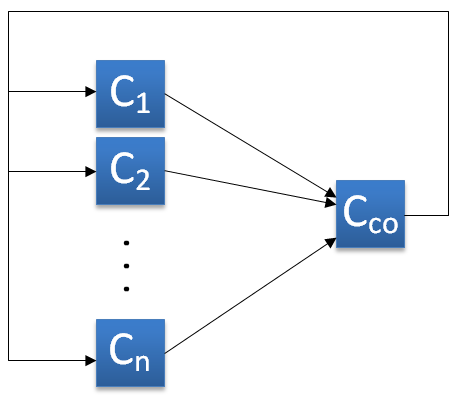
\includegraphics[width=\textwidth]{Figs/c_co.png}
		\caption{Components communicating via a central organising mechanism.}
		\label{fig:centralOrganizer}
	\end{subfigure}
	\begin{subfigure}[t]{0.45\textwidth}
		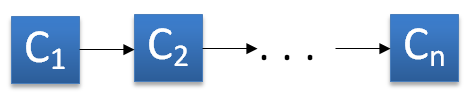
\includegraphics[width=\textwidth]{Figs/c_sequence.png}
		\caption{A sequence of components.}
		\label{fig:c_sequence}
	\end{subfigure}
\end{figure}
